
% v2-acmsmall-sample.tex, dated March 6 2012
% This is a sample file for ACM small trim journals
%
% Compilation using 'acmsmall.cls' - version 1.3 (March 2012), Aptara Inc.
% (c) 2010 Association for Computing Machinery (ACM)
%
% Questions/Suggestions/Feedback should be addressed to => "acmtexsupport@aptaracorp.com".
% Users can also go through the FAQs available on the journal's submission webpage.
%
% Steps to compile: latex, bibtex, latex latex
%
% For tracking purposes => this is v1.3 - March 2012
\documentclass[prodmode,acmtecs]{acmsmall} % Aptara syntax
\usepackage[spanish,polish]{babel}
\usepackage[T1]{fontenc}
\usepackage{fancyvrb}
\usepackage{graphicx,hyperref}
\newcommand\cutout[1]{}


\usepackage[table]{xcolor}
\usepackage[utf8]{inputenc}
\usepackage[parfill]{parskip}
\usepackage{tabulary}
\PassOptionsToPackage{hyphens}{url}
\usepackage{hyperref}    
\usepackage[capitalize]{cleveref}


% Metadata Information
% !!! TODO: SET THESE VALUES !!!
\acmVolume{0}
\acmNumber{0}
\acmArticle{CFP}
\acmYear{0}
\acmMonth{0}

\newcounter{colstart}
\setcounter{page}{4}

\RecustomVerbatimCommand{\VerbatimInput}{VerbatimInput}%
{
%fontsize=\footnotesize,
fontfamily=\rmdefault
}


\newcommand{\UnderscoreCommands}{%\do\verbatiminput%
\do\citeNP \do\citeA \do\citeANP \do\citeN \do\shortcite%
\do\shortciteNP \do\shortciteA \do\shortciteANP \do\shortciteN%
\do\citeyear \do\citeyearNP%
}

\usepackage[strings]{underscore}



% Document starts
\begin{document}


\setcounter{colstart}{\thepage}

\acmArticle{CFP}
\title{\huge\sc SIGLOG Monthly 232}
\author{DAVID PURSER\affil{University of Warsaw, Poland}
\vspace*{-2.6cm}\begin{flushright}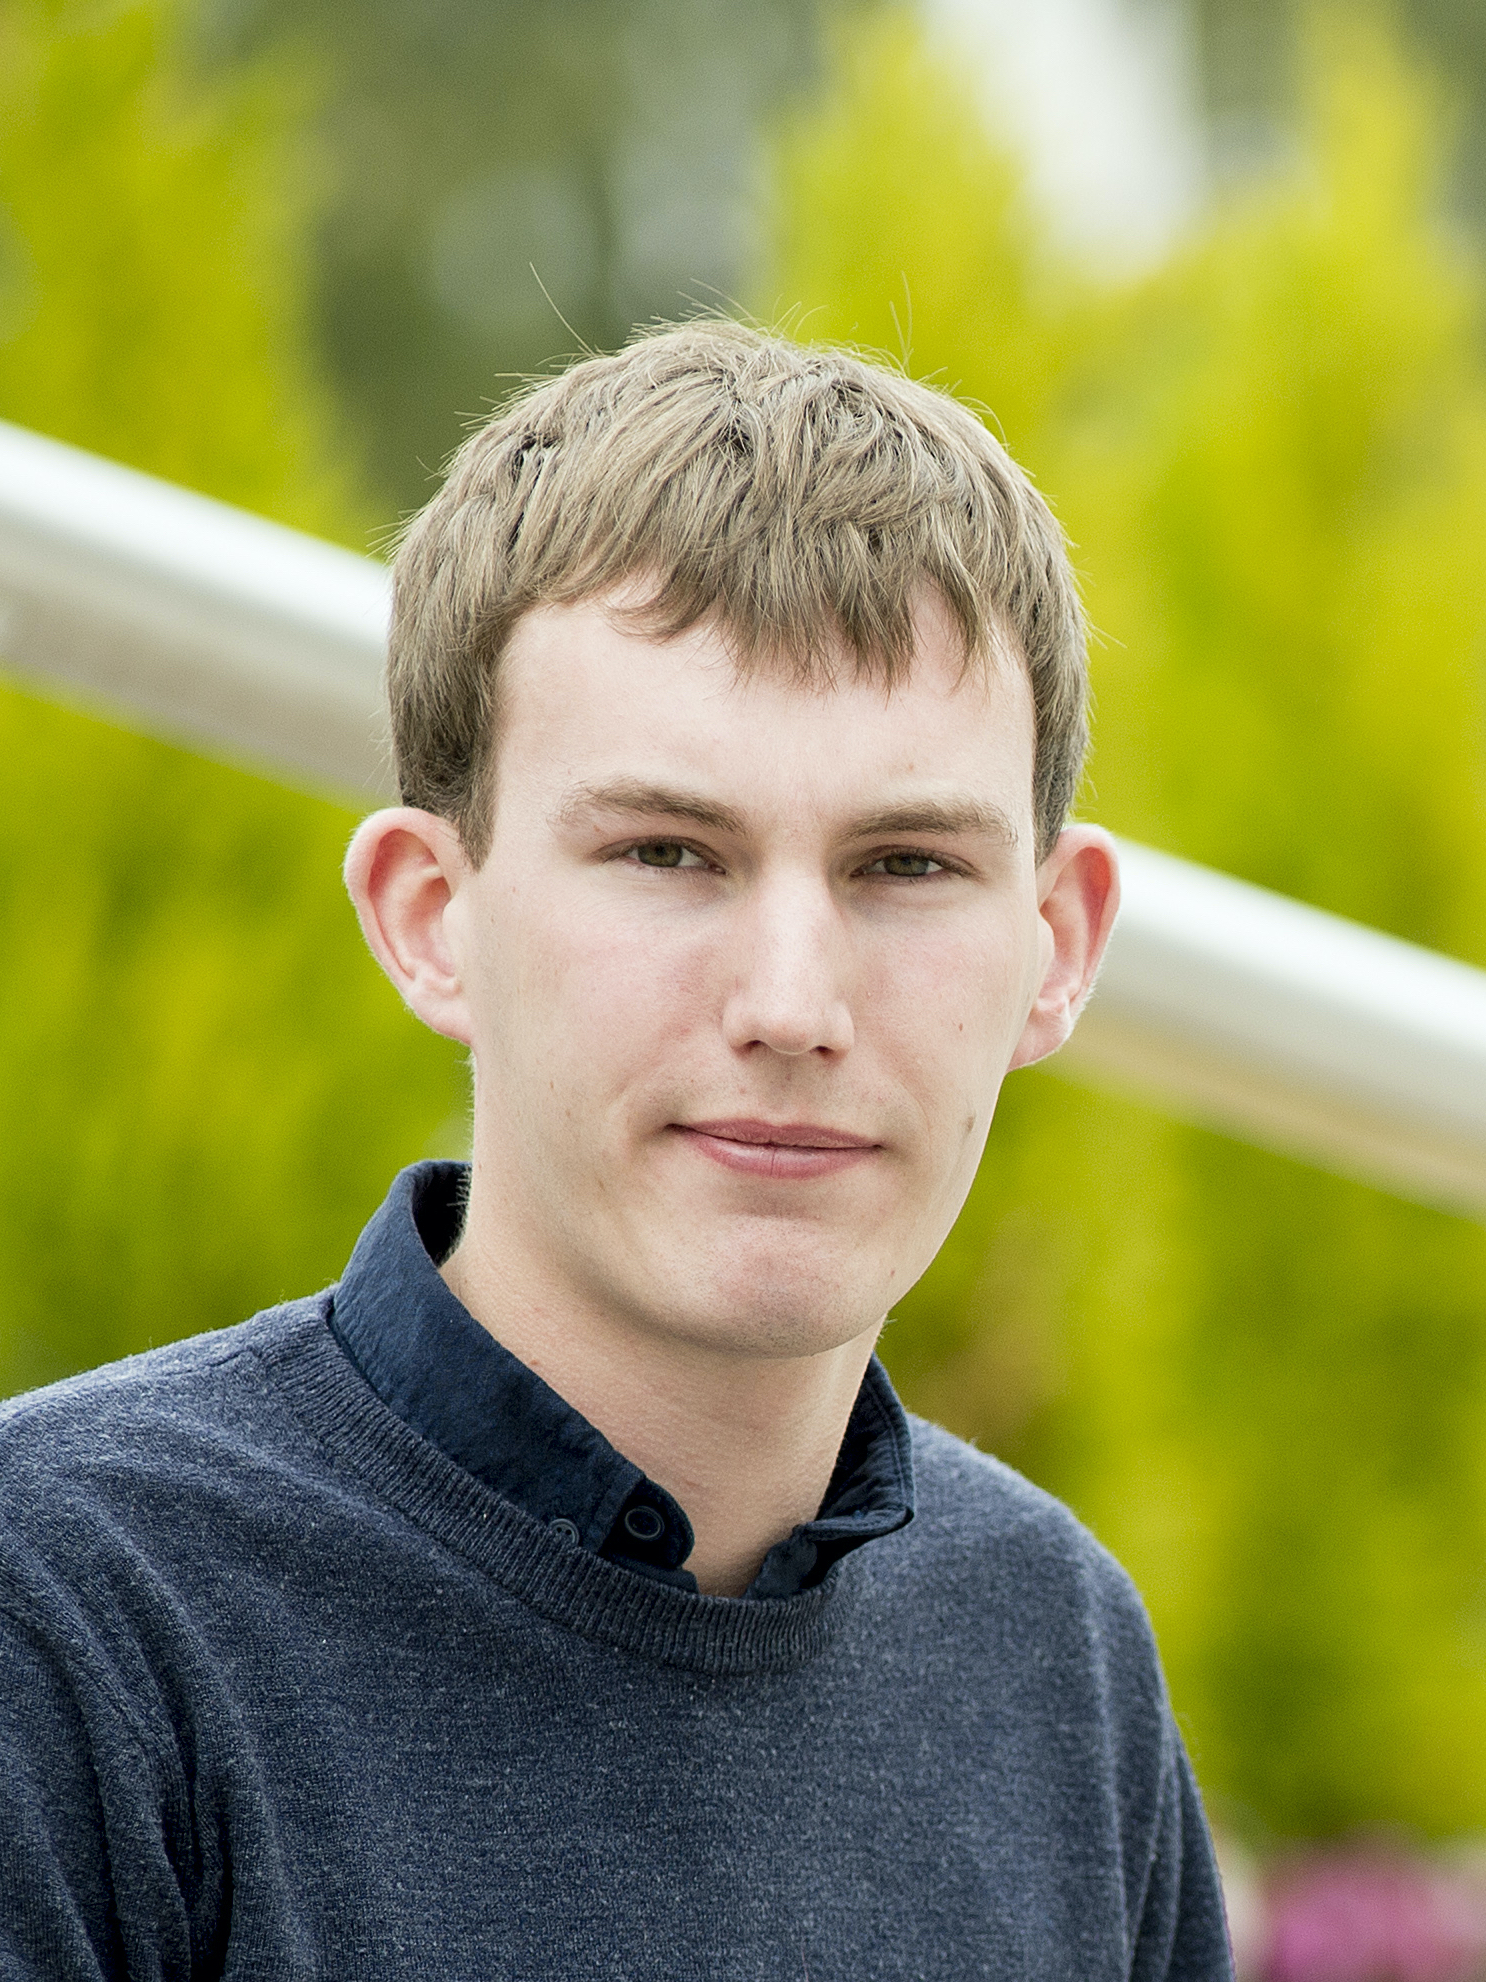
\includegraphics[width=30mm]{dp}\end{flushright}
}

\maketitlee

\href{https://lics.siglog.org/newsletters/}{Past Issues}
 - 
\href{https://lics.siglog.org/newsletters/inst.html}{How to submit an announcement}
\section{Table of Content}\begin{itemize}\item DEADLINES (\cref{deadlines}) 
 
\item ANNOUNCEMENTS 
 
\begin{itemize}\item Winner of the 2022 Ackermann Award (\cref{Winnerofthe2022AckermannAward})
\end{itemize} 
\item CALLS 
 
\begin{itemize}\item FSCD-CADE (CALL FOR WORKSHOP AND TUTORIAL PROPOSALS) (\cref{FSCDCADE})
\item STAF 2023 (CALL FOR WORKSHOP PROPOSALS) (\cref{STAF2023})
\item ICLP 2023 (CALL FOR PAPERS) (\cref{ICLP2023})
\item FSCD 2023 (CALL FOR PAPERS) (\cref{FSCD2023})
\item CONFEST 2023 (CALL FOR WORKSHOP PROPOSALS) (\cref{CONFEST2023})
\item LOGIC COLLOQUIUM 2023 (CALL FOR PAPERS) (\cref{LOGICCOLLOQUIUM2023})
\end{itemize} 
\item JOB ANNOUNCEMENTS 
 
\begin{itemize}\item PostDoc position in automata theory / algorithmic game theory, University of Warsaw (\cref{PostDocpositioninautomatatheoryalgorithmicgametheoryUniversityofWarsaw})
\end{itemize} 
\end{itemize}\section{Deadlines}\label{deadlines}\rowcolors{1}{white}{gray!25}\begin{tabulary}{\linewidth}{LL}PODS 2023:  & Dec 05, 2022 (Full paper) \\
Faculty Position at Cambridge:  & Dec 05, 2022 (Application deadline) \\
Oxford Faculty Positions:  & Dec 14, 2022 at noon (Application deadline) \\
FSCD-CADE:  & Dec 18, 2022 (Workshop proposal) \\
STAF 2023:  & Dec 20, 2022 (Workshop proposal) \\
PostDoc in automata/games, Warsaw:  & Dec 20, 2022 (Application deadline) \\
LICS 2023:  & Jan 18, 2023 (Titles and Short Abstracts Due), Jan 23, 2023 (Full Papers Due) \\
ICLP 2023:  & Jan 23, 2023 (Abstract registration), Jan 31, 2023 (Paper  (regular, applications, thematic tracks)), Apr 28, 2023 (Paper  (other paper types)) \\
FSCD 2023:  & Jan 30, 2023 (Abstract), Feb 03, 2023 (Paper) \\
Dov Gabbay Prize for Logic and Foundations:  & Jan 31, 2023 (Deadline for nominations) \\
S. Barry Cooper Prize:  & Jan 31, 2023 (Deadline for nominations) \\
CONFEST 2023:  & Feb 02, 2023 (Submission deadline) \\
CiE 2023:  & Feb 08, 2023 (Abstract), Feb 15, 2023 (Article) \\
ICALP 2023:  & Feb 11, 2023 at 11am CET (Paper) \\
LOGIC COLLOQUIUM 2023:  & Mar 01, 2023 (Abstract), Mar 01, 2023 (Student Travel Grants deadline) \\
\end{tabulary}
\section{Winner of the 2022 Ackermann Award}\label{Winnerofthe2022AckermannAward}ANNOUNCEMENT 

\begin{itemize}\item  The Ackermann Award 2021, the EACSL Outstanding Dissertation Award for Logic in Computer Science, is given to the PhD thesis: 
 
\begin{itemize}\item   Alexander Bentkamp: Superposition for Higher-Order Logic
\end{itemize} 
\item  The award will be presented at the 31st Computer Science Logic (CSL 2023) Conference, the annual meeting of the European Association for Computer Science Logic, February 13-16, 2023, in Warsaw, Poland. 
 
\item  A detailed report will be published in the proceedings of CSL 2023. 
 
\end{itemize}\section{FSCD-CADE}\label{FSCDCADE}  FSCD 2023 \href{https://easyconferences.eu/fscd2023/}{https://easyconferences.eu/fscd2023/} July 3-6, 2023\\ 
  CADE-29 \href{https://easyconferences.eu/cade2023/}{https://easyconferences.eu/cade2023/} July 1-4, 2023\\ 
  Rome, Italy\\ 
CALL FOR WORKSHOP AND TUTORIAL PROPOSALS 

\begin{itemize}\item  We invite proposals for workshops, tutorials or other satellite events, on any topic related to formal structures in computation, deduction and automated reasoning, from theoretical foundations to tools and applications. 
 
  FSCD satellite events will take place before the main conference on July 1-2, and CADE satellite events will take place after the main conference on July 4 (afternoon)-5. It is expected that satellite events would run for 1/2, 1 or 2 days (max 1 and 1/2 day for CADE satellite events), and be open to participants of parallel events. Please note overlaps between FSCD workshops and CADE conference and between CADE workshops and FSCD conference (see Important Dates below). 
 
\item  PROPOSALS 
 
  For proposal submission information, please see \href{https://easyconferences.eu/cade2023/call-for-workshops-tutorial-proposals/}{https://easyconferences.eu/cade2023/call-for-workshops-tutorial-proposals/} 
 
\item  IMPORTANT DATES 
 
\rowcolors{1}{white}{gray!25}\begin{tabulary}{\linewidth}{LL}CADE:  & July 1-4, 2023 \\
FSCD:  & July 3-6, 2023 \\
CADE Workshops:  & July 4 (afternoon) and 5, 2023 \\
FSCD Workshops:  & July 1-2, 2023 \\
Workshop proposal submission:  & Dec 18, 2022 \\
Notification of success of proposals:  & Dec 23, 2022 \\
\end{tabulary}
 
\end{itemize}\section{STAF 2023: Software Technologies Applications and Foundations }\label{STAF2023}  Leicester, UK, between July 17-21\\ 
  \href{https://conf.researchr.org/home/staf-2023}{https://conf.researchr.org/home/staf-2023}\\ 
CALL FOR WORKSHOP PROPOSALS 

\begin{itemize}\item   Software Technologies: Applications and Foundations (STAF) is a federation of leading conferences on software technologies. It was formed after the end of the successful TOOLS federated event in 2012, providing an umbrella organisation, with a steering committee that aims to provide continuity. The STAF federated event runs annually; the conferences that participate may vary from year to year, but all focus on practical and foundational advances in software technology. The conferences address all aspects of software technology, from object-oriented design, testing, formal approaches to modelling and verification, transformation, model-driven engineering, aspect-oriented techniques, and tools. 
 
  The workshops at STAF will provide a collaborative forum for groups of typically 15 to 35 participants to exchange recent and/or preliminary results, to conduct intensive discussions on a particular topic, or to coordinate efforts between representatives of a technical community. They are intended as a forum for lively discussion on innovative ideas, recent progress, or practical experience on specific aspects, specific problems, or domain-specific needs. Each workshop should provide a balanced distribution of its time for both presentation of papers and discussions. We encourage prospective workshop organisers to submit proposals for highly-interactive workshops. Both research-oriented and applied topics are welcome. The duration of each workshop is either half day or full day. 
 
\item  IMPORTANT DATES 
 
\rowcolors{1}{white}{gray!25}\begin{tabulary}{\linewidth}{LL}Workshop proposal submission:  & Dec 20, 2022 \\
Notification of acceptance of workshop proposals:  & Jan 10, 2023 \\
\end{tabulary}
 
\item  For details and submission instructions see:  \href{https://conf.researchr.org/track/staf-2023/staf-2023-workshops}{https://conf.researchr.org/track/staf-2023/staf-2023-workshops} 
 
\end{itemize}\section{ICLP 2023: 39TH INTERNATIONAL CONFERENCE ON LOGIC PROGRAMMING}\label{ICLP2023}  London, United Kingdom (in-person)\\ 
  July 9-15, 2023\\ 
  \href{https://iclp2023.imperial.ac.uk/}{https://iclp2023.imperial.ac.uk/} \\ 
CALL FOR PAPERS 

\begin{itemize}\item  SCOPE 
 
  Since the first conference held in Marseille in 1982, ICLP has been the premier international event for presenting research in logic programming. Contributions are sought in all areas of logic programming, including but not restricted to: 
 
\begin{itemize}\item  Theoretical Foundations.
\item  Language Design and Programming Methodologies.
\item  Program Analysis and Optimization.
\item  Implementation Methodologies.
\item  Related Paradigms, Integration, and Synergies.
\item  Applications of Logic Programming.  
\end{itemize} 
\item  IMPORTANT DATES 
 
\rowcolors{1}{white}{gray!25}\begin{tabulary}{\linewidth}{LL}Abstract registration:  & Jan 23, 2023 \\
Paper submission (regular, applications, thematic tracks):  & Jan 31, 2023 \\
Notification to authors:  & Feb 28, 2023 \\
Revision submission (TPLP papers):  & Mar 20, 2023 \\
Paper submission (other paper types):  & Apr 28, 2023 \\
Workshop proposals:  & Mar 20, 2023 \\
Final notifications (all paper kinds):  & May 19, 2023 \\
Camera-ready copy due (all paper kinds):  & May 26, 2023 \\
Conference:  & Jul 9-15, 2023 \\
\end{tabulary}
 
  Deadlines expire at the end of the day, anywhere on earth. 
 
\item  TRACKS AND SPECIAL SESSIONS 
 
  Besides the main track, ICLP 2023 will host additional tracks: 
 
\begin{itemize}\item  Applications Track: we invite submissions of papers on emerging and deployed applications of LP, describing all aspects of the development, deployment, and evaluation of logic programming systems to solve real-world problems, including interesting case studies and benchmarks, and discussing lessons learned.
\item  Thematic Tracks: we invite submissions to two thematic tracks, exploring specific roles and potential for logic programming; these thematic tracks are: Logic Programming and Machine Learning and Logic Programming and Explainability, Ethics, and Trustworthiness
\item  Recently Published Research Track: this track provides a forum to discuss important results related to logic programming that appeared recently (from January 2021 onwards) in selective journals and conferences, but have not been previously presented at ICLP.
\item  System Demonstrations: we invite submissions showcasing logic programming systems and implementations in a live setting. This track is not designed to be sales pitches, demonstrations are a way for the community to see the relevance, potential, and innovation of the tool and allow time for discussion with its creator.
\item  Birds-of-a-Feather (BoF) sessions: we invite proposals for sessions meant to provide an inclusive environment for colleagues with similar interests to meet for informal discussion. Proposers of BoF sessions should serve as discussion leaders only. BoFs are not intended to be presentations.
\end{itemize} 
  In addition,  ICLP 2023 will host: 
 
\begin{itemize}\item  Doctoral Consortium and Mentoring Sessions: the Doctoral Consortium (DC) on Logic Programming provides students and early career researchers with the opportunity to present and discuss their research directions, obtain feedback from both peers and experts in the field, and participate in mentoring sessions on how to prepare and succeed for a research career. We will have leaders in logic programming research from academia and industry to give invited talks on their research areas. The best paper from the DC will be given the opportunity to make a presentation in a session of the main ICLP conference.
\item  Tutorials.
\item  Co-located Workshops.
\item  Summer School on Logic Programming.
\item  Logic Programming Contest.
\end{itemize} 
\item  SUBMISSION DETAILS 
 
  See \href{https://iclp2023.imperial.ac.uk/calls}{https://iclp2023.imperial.ac.uk/calls} for further details and specific instructions for each track on the respecitve subpages. 
 
\item  Any additional question can be directed towards the ICLP Chairs: iclp2023@easychair.org 
 
\end{itemize}\section{FSCD 2023: 8th International Conference on Formal Structures for Computation and Deduction}\label{FSCD2023}  July 3-6, 2023, Rome, Italy\\ 
  \href{https://easyconferences.eu/fscd2023/}{https://easyconferences.eu/fscd2023/}\\ 
  In-cooperation with ACM SIGLOG and SIGPLAN\\ 
CALL FOR PAPERS 

\begin{itemize}\item  IMPORTANT DATES 
 
  All deadlines are midnight anywhere-on-earth (AoE); late submissions will not be considered. 
 
\rowcolors{1}{white}{gray!25}\begin{tabulary}{\linewidth}{LL}Abstract:  & Jan 30, 2023 \\
Paper submission:  & Feb 03, 2023 \\
Rebuttal:  & Mar 24-28, 2023 \\
Notification:  & Apr 13, 2023 \\
Final version:  & Apr 27, 2023 \\
\end{tabulary}
 
\item  OVERVIEW 
 
  FSCD (\href{https://fscd-conference.org/}{https://fscd-conference.org/}) covers all aspects of formal structures for computation and deduction from theoretical foundations to applications. Building on two communities, RTA (Rewriting Techniques and Applications) and TLCA (Typed Lambda Calculi and Applications), FSCD embraces their core topics and broadens their scope to closely related areas in logic, models of computation, semantics and verification in new challenging areas. 
 
  The suggested, but not exclusive, list of topics for submission is:  
 
\begin{itemize}\item  Calculi: Rewriting systems (string, term, higher-order, graph, conditional, modulo, infinitary, etc.); Lambda calculus; Logics (first-order, higher-order, equational, modal, linear, classical, constructive, etc.); Proof theory (natural deduction, sequent calculus, proof nets, etc.); Type theory and logical frameworks; Homotopy type theory; Quantum calculi.
\item  Methods in Computation and Deduction: Type systems (polymorphism, dependent, recursive, intersection, session, etc.); Induction, coinduction; Matching, unification, completion, orderings; Strategies (normalization, completeness, etc.); Tree automata; Model building and model checking; Proof search and theorem proving; Constraint solving and decision procedures.
\item  Semantics: Operational semantics and abstract machines; Game Semantics and applications; Domain theory and categorical models; Quantitative models (timing, probabilities, etc.); Quantum computation and emerging models in computation.
\item  Algorithmic Analysis and Transformations of Formal Systems: Type inference and type checking; Abstract Interpretation; Complexity analysis and implicit computational complexity; Checking termination, confluence, derivational complexity and related properties; Symbolic computation.
\item  Tools and Applications: Programming and proof environments; Verification tools; Proof assistants and interactive theorem provers; Applications in industry; Applications of formal systems in other sciences; Applications of formal systems in education.
\item  Formal Systems for Semantics and Verification in new challenging areas: Certification; Security; Blockchain protocols; Data bases; Deep learning and machine learning algorithms; Planning.
\end{itemize} 
\item  SPECIAL ISSUE 
 
  We aim to have a special issue of Logical Methods in Computer Science of selected papers. More details will be provided later. 
 
\item  BEST PAPER AWARD BY JUNIOR RESEARCHERS 
 
  The program committee will select a paper in which at least one author is a junior researcher, i.e. either a student or whose PhD award date is less than three years from the first day of the meeting. When submitting the paper, other authors should declare to the PC Chair that at least 50% of contribution is made by the junior researcher(s).  
 
\item  See full call for papers for submission and publication information: \href{https://easyconferences.eu/fscd2023/cfp/}{https://easyconferences.eu/fscd2023/cfp/} 
 
\end{itemize}\section{CONFEST 2023}\label{CONFEST2023}  September 18-23, 2023, Antwerpen, Belgium\\ 
  \href{https://www.uantwerpen.be/en/conferences/confest-2023/}{https://www.uantwerpen.be/en/conferences/confest-2023/}\\ 
CALL FOR WORKSHOP PROPOSALS 

\begin{itemize}\item  CONFEST is an umbrella conference comprising four international meetings: 
 
\begin{itemize}\item  CONCUR (34th International Conference on Concurrency Theory),
\item  QEST (20th International Conference on Quantitative Evaluation of SysTems),
\item  FORMATS (21st International Conference on Formal Modeling and Analysis of Timed Systems), and
\item  FMICS (28th International Conference on Formal Methods for Industrial Critical Systems).
\end{itemize} 
\item   Researchers and practitioners are invited to submit proposals for ONE DAY workshops on topics related to theory, formal modeling, verification,performance evaluation and engineering of concurrent, timed, industrial,and other systems.Typically, CONFEST workshops feature a number of invited speakers and anumber of contributed presentations. 
 
  The workshops will take place one day before (18 September) and one day after (23 September) the main conferences. 
 
\item  TOPICS 
 
  The purpose of the workshops is to provide participants with a friendly, stimulating, and interactive atmosphere for 
 
\begin{itemize}\item  presenting novel ideas,
\item  discussing their applications,
\item  encouraging cross-fertilization between industry and academia, and
\item  fostering opportunities for young and prospective researchers.
\end{itemize} 
\item  IMPORTANT DATES 
 
\rowcolors{1}{white}{gray!25}\begin{tabulary}{\linewidth}{LL}Submission deadline:  & Feb 02, 2023 \\
Notification:  & Feb 16, 2023 \\
Program of the workshops ready:  & Aug 16, 2023 \\
Workshops:  & Sep 18+23, 2023 \\
CONFEST conferences:  & Sep 18-23, 2023 \\
\end{tabulary}
 
\item  For details and submission instructions, see: \href{https://www.uantwerpen.be/en/conferences/confest-2023/workshops/call/}{https://www.uantwerpen.be/en/conferences/confest-2023/workshops/call/} 
 
\end{itemize}\section{LOGIC COLLOQUIUM 2023: European Summer Meeting of the Association for Symbolic Logic}\label{LOGICCOLLOQUIUM2023}  University of Milan, Italy\\ 
  June 5-9 2023\\ 
  \href{https://lc2023.unimi.it}{https://lc2023.unimi.it}\\ 
CALL FOR PAPERS 

\begin{itemize}\item  GENERAL INFORMATION 
 
  LOGIC COLLOQUIUM is the European Summer Meeting of the Association for Symbolic Logic (ASL) - \href{https://aslonline.org}{https://aslonline.org} - an international organization supporting research and critical studies in logic. LOGIC COLLOQUIUM is a venue for all researchers working in logic from computer science, mathematics, and philosophy. 
 
\item  IMPORTANT DATES 
 
\rowcolors{1}{white}{gray!25}\begin{tabulary}{\linewidth}{LL}Abstract submission:  & Mar 01, 2023 \\
Student Travel Grants deadline:  & Mar 01, 2023 \\
Notifications of Abstract Acceptance:  & Apr 03, 2023 \\
Decision on Travel Grants:  & Apr 05, 2023 \\
Deadline for Early Registration:  & May 01, 2023 \\
Registration closing:  & May 15, 2023 \\
Start of the Conference:  & Jun 05, 2023 \\
End of the Conference:  & Jun 09, 2023 \\
\end{tabulary}
 
\item  CONTRIBUTED TALKS 
 
  Online contributed talks are welcome and we will do our best to make this event hybrid, although we of course encourage you to come to Milan to meet the community. 
 
  Topics of interest include: 
 
\begin{itemize}\item  Set Theory
\item  Proof Theory
\item  Model Theory
\item  Computability Theory
\item  Philosophical Logic
\item  Logic in Computer Science
\end{itemize} 
  Please see submission instructions on the full call: \href{https://lc2023.unimi.it/call-for-papers/}{https://lc2023.unimi.it/call-for-papers/} 
 
\item  STUDENT TRAVEL GRANTS 
 
  To be considered for a travel award, please see the full call: \href{https://lc2023.unimi.it/call-for-papers/}{https://lc2023.unimi.it/call-for-papers/} 
 
\item  INVITED SPEAKERS 
 
\begin{itemize}\item  Gal Binyamini (Weizmann Institute of Science, Israel)
\item  Nicola Gambino (Department of Mathematics, University of Manchester, UK)
\item  Martino Lupini (Department of Mathematics, University of Bologna, Italy)
\item  Francesca Poggiolesi (Université Paris 1 Panthéon-Sorbonne, CNRS, Institut d’Histoire et de Philosophie des Sciences et des Techniques, France)
\item  Viorica Sofronie-Stokkermans (Institut für Informatik, University Koblenz-Landau, Germany)
\item  Igor Carboni Oliveira (Department of Computer Science, University of Warwick, UK)
\item  Zoltán Vidnyánszky (Institute of Mathematics, Eotvos University, Hungary)
\item  Gabriel Goldberg (Mathematics, UCBerkeley, USA)
\item  Johanna Franklin (Department of Mathematics, Hofstra University, USA)
\end{itemize} 
\item  TUTORIAL SPEAKERS 
 
\begin{itemize}\item  Itay Kaplan (Einstein Institute of Mathematics, Hebrew University of Jerusalem, Israel)
\end{itemize} 
  MORE TUTORIAL SPEAKERS T.B.A. 
 
\item  SPECIAL SESSIONS 
 
  Logic Colloquium 2023 will feature 6 special sessions, the topics of which are to be announced. 
 
\end{itemize}\section{PostDoc position in automata theory / algorithmic game theory, University of Warsaw}\label{PostDocpositioninautomatatheoryalgorithmicgametheoryUniversityofWarsaw}JOB ANNOUNCEMENT 

\begin{itemize}\item  DETAILS 
 
\begin{itemize}\item  Application deadline: December 20, 2022
\item  Starting date: Flexible
\item  Salary: 7600 PLN/month before taxes (quite competitive in Poland)
\item  Duration: 6 or 12 months
\item  Project: ``Computational aspects of infinite-duration games'' funded by NCN
\item  Principal investigator: Paweł Parys (www.mimuw.edu.pl/~parys)
\item  Contact: parys@mimuw.edu.pl
\end{itemize} 
\item  The project concerns solving parity games and other kind of games, and related questions. This is mostly a theoretical research. We promise a vibrant working atmosphere in the automata group at the University of Warsaw, and exciting and challenging research problems. 
 
\item  The ideal candidate is expected to have: 
 
\begin{itemize}\item  PhD degree or equivalent in computer science or math (finished or to be
\end{itemize} 
  finished soon), 
 
\begin{itemize}\item  solid background in formal methods and automata theory,
\item  significant publication record,
\item  strong motivation for research work in foundations of computer science,
\item  advanced skills in written and spoken English.
\end{itemize} 
\item  To apply, please send your curriculum vitae to parys@mimuw.edu.pl. 
 
\end{itemize}


To the \href{http://siglog.org/}{SIGLOG} or \href{https://lics.siglog.org}{LICS} website\end{document}